\chapter{Cơ sở Lý thuyết và Phương pháp luận Toán học}
\label{chap:theoretical_foundations}
\label{chap:foundations}

Chương này trình bày toàn bộ cơ sở lý thuyết, mô hình biểu diễn hình học, cơ chế căn chỉnh không gian, phân phối nhiễu nền thực nghiệm và khung suy luận kinh tế lượng cho bài toán lượng hóa trôi dạt biểu diễn (Representation Drift) trên Đồ thị Tri thức Động (Evolving Knowledge Graph -- EKG). Toàn bộ hệ thống phương pháp luận được thiết kế tuân thủ nghiêm ngặt các tiên đề bảo toàn tính toàn vẹn thời gian, triệt tiêu nội sinh thống kê và cung cấp độ tin cậy suy luận tối đa.

% ==============================================================================
% 2.1 MÔ HÌNH THỜI GIAN VÀ TÍNH TOÀN VẸN THỜI GIAN
% ==============================================================================
\section{Mô hình Thời gian và Tính Toàn vẹn Thời gian}
\label{sec:temporal_model_integrity}

\subsection{Khái niệm Đồ thị Tri thức Động (Evolving Knowledge Graph)}
Đồ thị tri thức động là một chuỗi các trạng thái đồ thị tri thức biến đổi theo thời gian thực. Tại mỗi mốc thời gian rời rạc $t \in \{1, 2, \dots, T\}$, trạng thái đồ thị được biểu diễn bởi một bộ ba thành phần:
\begin{equation}
\mathcal{G}_t = \left(\mathcal{E}_t, \mathcal{R}_t, \mathcal{T}_t\right)
\end{equation}
trong đó:
\begin{itemize}
    \item $\mathcal{E}_t \subset \mathcal{E}$ là tập hữu hạn các thực thể (entities) tồn tại và đã được phân giải tại thời điểm $t$.
    \item $\mathcal{R}_t \subset \mathcal{R}$ là tập các quan hệ ngữ nghĩa (relations) có hiệu lực tại thời điểm $t$.
    \item $\mathcal{T}_t \subseteq \mathcal{E}_t \times \mathcal{R}_t \times \mathcal{E}_t$ là tập các bộ ba tri thức sự thật (facts/triples) dạng $\tau = (h, r, t)$ với $h$ là thực thể đầu (head), $r$ là quan hệ (relation), và $t$ là thực thể cuối (tail).
\end{itemize}

Trong quá trình tiến hóa thực tế của tri thức nhân loại, đồ thị tri thức phát triển qua các thao tác: bổ sung thực thể mới ($\mathcal{E}_{t-1} \subset \mathcal{E}_t$), cập nhật hoặc bãi bỏ các mối quan hệ ngữ nghĩa, và tái cấu trúc liên kết topo giữa các node.

\subsection{Trục Thời gian Tam phân (Three-Way Temporal Axis Separation)}
Một trong những nguyên nhân hàng đầu dẫn đến hiện tượng rò rỉ dữ liệu (data leakage) và ngụy tạo kết quả trong các nghiên cứu về đồ thị tri thức biến đổi theo thời gian là sự nhầm lẫn giữa các trục thời gian khác nhau. Đề tài thiết lập một quy tắc phân tách nghiêm ngặt ba trục thời gian độc lập:

\begin{enumerate}
    \item \textbf{Trục Hiệu lực Thế giới Thực (World Validity Axis):}
    Khoảng thời gian $[\tau_{\text{valid\_from}}, \tau_{\text{valid\_to}}]$ mô tả khoảng thời gian một sự kiện hoặc mối quan hệ thực sự tồn tại và đúng đắn trong thực tế khách quan.
    \item \textbf{Trục Ghi nhận Bằng chứng Công khai (Evidence Observation Axis):}
    Dấu thời gian $t_{\text{evidence}} \equiv \texttt{evidence\_observed\_at}$ là thời điểm phiên bản bằng chứng, bài báo hoặc tài liệu chứa đựng thông tin về bộ ba tri thức được công bố công khai lần đầu tiên trên các nguồn dữ liệu có thể kiểm chứng độc lập. Đây là trục thời gian khoa học quyết định việc một sự thật có được phép đưa vào đồ thị tại mốc cắt hay không.
    \item \textbf{Trục Thu thập Kỹ thuật (Project Acquisition Axis):}
    Dấu thời gian $t_{\text{crawl}} \equiv \texttt{retrieved\_at\_real}$ (hoặc $\texttt{ingested\_at\_real}$) ghi nhận thời điểm máy chủ thu thập dữ liệu (crawler) thực hiện tải và lưu trữ bản ghi vào hệ thống.
\end{enumerate}

\begin{definition}[Nguyên tắc Bất khả Hoán đổi]
Ba trục thời gian trên tuyệt đối không được phép hoán đổi hoặc suy diễn thay thế cho nhau:
\begin{equation}
[\tau_{\text{valid\_from}}, \tau_{\text{valid\_to}}] \neq t_{\text{evidence}} \neq t_{\text{crawl}}
\end{equation}
Một sự thật có thể đã đúng trong thế giới thực từ năm 2020 ($\tau_{\text{valid\_from}} = 2020$), nhưng bằng chứng chỉ được báo chí công bố vào ngày 15/01/2024 ($t_{\text{evidence}} = \text{2024-01-15}$), và hệ thống thu thập vào ngày 20/01/2024 ($t_{\text{crawl}} = \text{2024-01-20}$). Việc xây dựng trạng thái đồ thị tại mốc cắt $T_{\text{cutoff}}$ bắt buộc phải dựa hoàn toàn trên $t_{\text{evidence}}$.
\end{definition}

\subsection{Hệ Tiên đề Bất biến Thời gian Bất khả Xâm phạm}
Để đảm bảo tính hợp lệ khoa học và khả năng tái lập độc lập của mọi phép đo trôi dạt biểu diễn, quy trình nghiên cứu áp đặt hệ thống bất biến nghiêm ngặt:

\begin{axiom}[Bất biến Chống Rò rỉ Bằng chứng Tương lai -- INV-01]
Mọi bộ ba sự thật $\tau \in \mathcal{T}_t$ được đưa vào lát cắt đồ thị (snapshot) tại mốc cắt thời gian $T_{\text{cutoff}}$ bắt buộc phải thỏa mãn:
\begin{equation}
\texttt{evidence\_observed\_at}(\tau) \le T_{\text{cutoff}}
\end{equation}
Bất kỳ sự thật nào có bằng chứng được công bố sau $T_{\text{cutoff}}$ tuyệt đối bị cấm xuất hiện trong snapshot, ngay cả khi nó mô tả sự kiện đã xảy ra trong quá khứ.
\end{axiom}

\begin{axiom}[Bất biến Phân giải Thực thể Không Dùng Tri thức Tương lai -- INV-02]
Bảng ánh xạ đồng nhất thực thể (Entity Resolution Mapping) $M_t$ tại mốc cắt $T_{\text{cutoff}}$ chỉ được phép sử dụng các luật liên kết danh tính khả dụng tại hoặc trước thời điểm cắt:
\begin{equation}
\texttt{mapping\_available\_at}(m) \le T_{\text{cutoff}}, \quad \forall m \in M_t
\end{equation}
Không được phép sử dụng danh mục thực thể hoàn chỉnh ở tương lai để gộp hoặc phân giải các node trong quá khứ.
\end{axiom}

\begin{axiom}[Bất biến Bổ sung Bất khả Biến -- Append-Only Provenance -- INV-03]
Kho lưu trữ phiên bản sự thật ($\texttt{FactVersion}$) và kho văn bản thô hoạt động hoàn toàn theo cơ chế nối tiếp (append-only). Tuyệt đối cấm các thao tác xóa ($\texttt{DELETE}$), cắt tỉa ($\texttt{TRUNCATE}$) hoặc sửa đổi tại chỗ ($\texttt{UPDATE}$) dữ liệu lịch sử. Mọi sự thay đổi trạng thái phải được ghi nhận dưới dạng phiên bản mới cùng nguồn gốc xuất xứ (provenance) đầy đủ.
\end{axiom}

\begin{axiom}[Bất biến Tái lập Định cảm -- Deterministic Rebuild -- INV-04]
Với cùng một tập dữ liệu đầu vào đã khóa, cùng mã nguồn đã định danh commit, cùng bộ tham số cấu hình và các giá trị seed ngẫu nhiên cố định, quy trình tái sinh snapshot và huấn luyện phải tạo ra các tệp cấu trúc có mã băm cryptographic SHA-256 trùng khớp từng byte:
\begin{equation}
\text{SHA-256}\left(\text{Pipeline}(\mathcal{D}, \text{Config}, \text{Seed})\right) \equiv \text{Hằng số}
\end{equation}
\end{axiom}

% ==============================================================================
% 2.2 MÔ HÌNH BIỂU DIỄN TRI THỨC TRANSE-L2
% ==============================================================================
\section{Mô hình Biểu diễn Tri thức TransE-L2}
\label{sec:transe_l2_kge}

\subsection{Không gian Biểu diễn Hình học}
Mô hình TransE \cite{bordes2013translating} nhúng các thực thể và quan hệ của đồ thị tri thức vào một không gian vector liên tục $d$-chiều Euclidean thực:
\begin{equation}
\mathbf{h}, \mathbf{t} \in \mathbb{R}^d, \quad \mathbf{r} \in \mathbb{R}^d
\end{equation}
Trong nghiên cứu này, chiều không gian biểu diễn được ấn định chặt chẽ tại $d = 64$ dựa trên các kết quả khảo sát thực nghiệm (pilot studies) nhằm đảm bảo cân bằng tối ưu giữa năng lực biểu diễn cấu trúc đồ thị và tính ổn định hình học khi căn chỉnh trực giao.

\subsection{Giả thuyết Tịnh tiến Vector và Hàm Năng lượng L2}
Triết lý cốt lõi của TransE là xem quan hệ ngữ nghĩa $r$ như một phép tịnh tiến vector từ thực thể đầu $h$ đến thực thể cuối $t$:
\begin{equation}
\mathbf{h} + \mathbf{r} \approx \mathbf{t}
\end{equation}
Mức độ tương thích của một bộ ba ứng viên $\tau = (h, r, t)$ được đo lường thông qua hàm năng lượng khoảng cách Euclid $L_2$:
\begin{equation}
E(h, r, t) = \|\mathbf{h} + \mathbf{r} - \mathbf{t}\|_2 = \sqrt{\sum_{k=1}^d \left(h_k + r_k - t_k\right)^2}
\end{equation}
Một bộ ba hợp lệ trong đồ thị tri thức sẽ có mức năng lượng $E(h, r, t)$ tiệm cận 0, trong khi các bộ ba sai hoặc không tồn tại sẽ có giá trị năng lượng lớn.

\subsection{Hàm Mất mát Margin Ranking Loss và Tối ưu hóa}
Để huấn luyện mô hình TransE, nghiên cứu áp dụng hàm mất mát xếp hạng biên có điều chuẩn (Margin Ranking Loss):
\begin{equation}
\mathcal{L} = \sum_{(h,r,t) \in \mathcal{T}^+} \sum_{(h',r,t') \in \mathcal{T}^-} \max\left(0, \gamma + E(h,r,t) - E(h',r,t')\right) + \lambda \sum_{e \in \mathcal{E}} \|\mathbf{e}\|_2^2
\label{eq:margin_ranking_loss}
\end{equation}
trong đó:
\begin{itemize}
    \item $\mathcal{T}^+$ là tập hợp các bộ ba sự thật dương (positive triples) có trong snapshot đồ thị $\mathcal{G}_t$.
    \item $\mathcal{T}^-$ là tập các bộ ba tiêu cực (negative triples) được tạo ra thông qua cơ chế lấy mẫu thay thế thực thể (Corrupted Triples):
    \begin{equation}
    \mathcal{T}^- = \{(h', r, t) \mid h' \in \mathcal{E}, (h', r, t) \notin \mathcal{T}^+\} \cup \{(h, r, t') \mid t' \in \mathcal{E}, (h, r, t') \notin \mathcal{T}^+\}
    \end{equation}
    \item $\gamma > 0$ là tham số biên (margin separator), được cố định tại $\gamma = 1.0$.
    \item $\lambda$ là trọng số điều chuẩn trọng lượng vector (regularization weight).
\end{itemize}

\begin{algorithm}[H]
\caption{Quy trình lấy mẫu tiêu cực có kiểm tra sự thật dương (Filtered Negative Sampling)}
\label{alg:negative_sampling}
\begin{algorithmic}[1]
\Require Bộ ba dương $(h, r, t) \in \mathcal{T}^+$, danh mục thực thể $\mathcal{E}$, tập sự thật $\mathcal{T}^+$, số lần thử tối đa $K=100$.
\State Tung đồng xu ngẫu nhiên Bernoulli $p \sim \text{Bernoulli}(0.5)$.
\For{$k = 1 \to K$}
    \If{$p == 1$} \Comment{Thay thế thực thể đầu}
        \State Chọn ngẫu nhiên $h' \sim \text{Uniform}(\mathcal{E})$.
        \If{$(h', r, t) \notin \mathcal{T}^+$} \Return $(h', r, t)$ \EndIf
    \Else \Comment{Thay thế thực thể cuối}
        \State Chọn ngẫu nhiên $t' \sim \text{Uniform}(\mathcal{E})$.
        \If{$(h, r, t') \notin \mathcal{T}^+$} \Return $(h, r, t')$ \EndIf
    \EndIf
\EndFor
\State \Return Bỏ qua mẫu nếu vượt quá $K$ lần thử (Fail-closed / Skip sample).
\end{algorithmic}
\end{algorithm}

Quá trình tối ưu hóa được thực hiện bằng giải thuật Stochastic Gradient Descent (SGD) từng bộ ba (per-triple SGD) với kích thước mini-batch danh nghĩa $B = 32$, tốc độ học (learning rate) $\eta = 0.01$, trải qua $E = 50$ epochs. Sau mỗi bước cập nhật trọng số, các vector embedding của thực thể được chiếu ngược lại mặt cầu đơn vị để ngăn chặn việc tối ưu hóa tầm thường bằng cách vô hạn hóa chuẩn vector:
\begin{equation}
\mathbf{e} \leftarrow \frac{\mathbf{e}}{\max\left(1, \|\mathbf{e}\|_2\right)}, \quad \forall e \in \mathcal{E}
\end{equation}

% ==============================================================================
% 2.3 CĂN CHỈNH KHÔNG GIAN BẰNG CENTERED ORTHOGONAL PROCRUSTES SVD
% ==============================================================================
\section{Căn chỉnh Không gian bằng Centered Orthogonal Procrustes SVD}
\label{sec:procrustes_alignment}

\subsection{Bản chất Tùy ý Tọa độ trong Huấn luyện KGE}
Mặc dù hàm mất mát \eqref{eq:margin_ranking_loss} ràng buộc khoảng cách tương đối giữa các vector, không gian biểu diễn Euclidean của KGE có tính bất biến quay và phản chiếu. Hai phiên bản huấn luyện độc lập với cùng một cấu hình mô hình nhưng khác biệt về seed ngẫu nhiên hoặc được huấn luyện trên hai snapshot liên tiếp sẽ tạo ra các hệ trục tọa độ hoàn toàn lệch pha:
\begin{equation}
\mathbf{e}^{(1)} \neq \mathbf{e}^{(2)} \quad \text{dù cấu trúc đồ thị không đổi.}
\end{equation}
Do đó, việc so sánh trực tiếp khoảng cách vector thô giữa hai không gian để kết luận về trôi dạt ngữ nghĩa là hoàn toàn phi khoa học. Cần thiết phải thiết lập một phép biến đổi đẳng cự (isometric mapping) để đưa hai không gian về cùng một hệ quy chiếu chung thông qua bài toán Orthogonal Procrustes cổ điển~\cite{schonemann1966generalized}.

\subsection{Bài toán Centered Orthogonal Procrustes}
Giả sử cần căn chỉnh không gian nguồn $S$ (với ma trận embedding $X$) sang không gian đích $T$ (với ma trận embedding $Y$). Để tránh việc phép biến đổi bị chi phối bởi các thực thể biến động cấu trúc mạnh, phép căn chỉnh được ước lượng độc quyền trên tập hợp các thực thể neo cố định (Persistent Anchor Entities):
\begin{equation}
\mathcal{A}_{\text{fit}} \subset \mathcal{E}_S \cap \mathcal{E}_T, \quad |\mathcal{A}_{\text{fit}}| = m_{\text{fit}} = 101
\end{equation}
Tập neo cố định này được lựa chọn độc lập từ trước và được kiểm định phân bố tách biệt hoàn toàn với tập neo đánh giá kiểm định (holdout anchors, $m_{\text{holdout}} = 66$).

Gọi $X_{\text{fit}} \in \mathbb{R}^{m \times d}$ và $Y_{\text{fit}} \in \mathbb{R}^{m \times d}$ là ma trận các vector embedding tương ứng của tập neo tại không gian nguồn và đích. Trọng tâm phân bố (centroids) của hai tập neo được xác định bởi:
\begin{equation}
\boldsymbol{\mu}_s = \frac{1}{m} \sum_{i=1}^m \mathbf{x}_i \in \mathbb{R}^d, \quad \boldsymbol{\mu}_t = \frac{1}{m} \sum_{i=1}^m \mathbf{y}_i \in \mathbb{R}^d
\end{equation}
Ma trận vector dịch tâm (centered matrices) được định nghĩa:
\begin{equation}
\widetilde{X} = X_{\text{fit}} - \mathbf{1}_m \boldsymbol{\mu}_s^T, \quad \widetilde{Y} = Y_{\text{fit}} - \mathbf{1}_m \boldsymbol{\mu}_t^T
\end{equation}
Bài toán Centered Orthogonal Procrustes tìm kiếm ma trận biến đổi trực giao tối ưu $Q \in \mathcal{O}(d)$ nhằm cực tiểu hóa sai số chuẩn Frobenius giữa hai tập điểm đã dịch tâm:
\begin{equation}
\min_{Q \in \mathbb{R}^{d \times d}} \left\| \widetilde{X} Q - \widetilde{Y} \right\|_F^2 \quad \text{sao cho} \quad Q^T Q = I_d
\label{eq:procrustes_opt}
\end{equation}

\subsection{Nghiệm Giải tích thông qua Phân tích Giá trị Kỳ dị (SVD)}
Khai triển bình phương chuẩn Frobenius trong hàm mục tiêu \eqref{eq:procrustes_opt}:
\begin{align}
\left\| \widetilde{X} Q - \widetilde{Y} \right\|_F^2 &= \text{Tr}\left( (\widetilde{X} Q - \widetilde{Y})^T (\widetilde{X} Q - \widetilde{Y}) \right) \nonumber \\
&= \text{Tr}\left( Q^T \widetilde{X}^T \widetilde{X} Q \right) - 2 \text{Tr}\left( Q^T \widetilde{X}^T \widetilde{Y} \right) + \text{Tr}\left( \widetilde{Y}^T \widetilde{Y} \right) \nonumber \\
&= \text{Tr}\left( \widetilde{X}^T \widetilde{X} \right) + \text{Tr}\left( \widetilde{Y}^T \widetilde{Y} \right) - 2 \text{Tr}\left( Q^T C \right)
\end{align}
với $C = \widetilde{X}^T \widetilde{Y} \in \mathbb{R}^{d \times d}$ là ma trận hiệp phương sai chéo giữa không gian nguồn và đích.

Do $\text{Tr}(\widetilde{X}^T \widetilde{X})$ và $\text{Tr}(\widetilde{Y}^T \widetilde{Y})$ là các hằng số độc lập với $Q$, việc cực tiểu hóa hàm sai số tương đương với việc cực đại hóa phần bù vết:
\begin{equation}
\max_{Q \in \mathcal{O}(d)} \text{Tr}\left( Q^T C \right)
\end{equation}
Thực hiện Phân tích Giá trị Kỳ dị (Singular Value Decomposition -- SVD) trên ma trận $C$:
\begin{equation}
C = U \Sigma V^T
\end{equation}
trong đó $U, V \in \mathcal{O}(d)$ là các ma trận trực giao và $\Sigma = \text{diag}(\sigma_1, \sigma_2, \dots, \sigma_d)$ với $\sigma_1 \ge \sigma_2 \ge \dots \ge \sigma_d \ge 0$.

Đặt $Z = V^T Q^T U \in \mathcal{O}(d)$. Khi đó:
\begin{equation}
\text{Tr}\left( Q^T C \right) = \text{Tr}\left( Q^T U \Sigma V^T \right) = \text{Tr}\left( V^T Q^T U \Sigma \right) = \text{Tr}\left( Z \Sigma \right) = \sum_{k=1}^d z_{kk} \sigma_k
\end{equation}
Do $Z$ là ma trận trực giao, mọi phần tử trên đường chéo thỏa mãn $|z_{kk}| \le 1$. Do đó, tổng vết đạt giá trị cực đại khi và chỉ khi $z_{kk} = 1, \forall k$, nghĩa là $Z = I_d$. Từ đó suy ra:
\begin{equation}
V^T Q^T U = I_d \implies Q^T = V U^T \implies Q^* = U V^T
\label{eq:procrustes_solution}
\end{equation}

\begin{remark}[Bảo vệ Tính Toàn vẹn Phản chiếu]
Trong không gian $d = 64$, nghiệm $Q^* = U V^T$ thuộc nhóm trực giao $\mathcal{O}(d)$ với $\det(Q^*) \in \{+1, -1\}$. Hệ thống kiểm tra nghiêm ngặt tính chất trực giao thông qua:
\begin{equation}
E_{\text{orth}} = \frac{1}{d} \| Q^T Q - I_d \|_F \le 10^{-4}, \quad \text{rank}(Q) = d = 64
\end{equation}
và kiểm tra khoảng cách dư trên tập kiểm định $m_{\text{holdout}}$:
\begin{equation}
\text{RMSE}_{\text{holdout}} = \sqrt{\frac{1}{m_{\text{holdout}}} \left\| \widetilde{X}_{\text{holdout}} Q^* - \widetilde{Y}_{\text{holdout}} \right\|_F^2} \le 2.0
\end{equation}
\end{remark}

\subsection{So sánh Khoa học: Affine Cosine vs. Centered Cosine}
Khi thực hiện đo lường độ dịch chuyển của một thực thể $e$ bất kỳ giữa hai không gian biểu diễn, tồn tại hai phương án toán học để định nghĩa độ bất đồng góc (angular dissimilarity):

\begin{definition}[Độ bất đồng Affine Cosine -- Đề cương gốc công thức 14 \& 26]
Biến đổi vector thực thể nguồn $\mathbf{x} \in \mathbb{R}^d$ thông qua ánh xạ affine trực giao đầy đủ vào không gian đích:
\begin{equation}
\mathbf{x}' = (\mathbf{x} - \boldsymbol{\mu}_s) Q^* + \boldsymbol{\mu}_t
\label{eq:affine_transform}
\end{equation}
Độ bất đồng Affine Cosine giữa vector nguồn sau chuyển đổi $\mathbf{x}'$ và vector đích $\mathbf{y}$ được xác định bởi:
\begin{equation}
d_{\text{aff}}(\mathbf{x}, \mathbf{y}) = 1 - \cos(\mathbf{x}', \mathbf{y}) = 1 - \frac{{\mathbf{x}'}^T \mathbf{y}}{\|\mathbf{x}'\|_2 \|\mathbf{y}\|_2}
\label{eq:affine_cosine}
\end{equation}
\end{definition}

\begin{definition}[Độ bất đồng Centered Cosine]
Đo lường sự biến dạng góc thuần túy của hai vector sau khi đã triệt tiêu toàn bộ độ lệch tâm phân bố:
\begin{equation}
\mathbf{x}_c = (\mathbf{x} - \boldsymbol{\mu}_s) Q^*, \quad \mathbf{y}_c = \mathbf{y} - \boldsymbol{\mu}_t
\end{equation}
\begin{equation}
d_{\text{cent}}(\mathbf{x}, \mathbf{y}) = 1 - \cos(\mathbf{x}_c, \mathbf{y}_c) = 1 - \frac{\mathbf{x}_c^T \mathbf{y}_c}{\|\mathbf{x}_c\|_2 \|\mathbf{y}_c\|_2}
\label{eq:centered_cosine}
\end{equation}
\end{definition}

\subsubsection{Phân tích Đối chiếu Bản chất Toán học}
Sự khác biệt cốt lõi giữa hai đại lượng này nằm ở cơ chế xử lý độ dịch chuyển tịnh tiến tuyệt đối (absolute spatial displacement):
\begin{enumerate}
    \item \textbf{Centered Cosine:} Có tính chất bất biến tịnh tiến toàn cục (translational invariance). Bằng cách trừ vector kỳ vọng tâm $\boldsymbol{\mu}_s$ và $\boldsymbol{\mu}_t$, phép đo này chỉ quan sát độ biến dạng hướng tương đối quanh tâm của đám mây điểm. Tuy nhiên, trong không gian nhúng của TransE, vị trí tâm của đồ thị phản ánh mật độ liên kết toàn cục; việc triệt tiêu hoàn toàn tọa độ tuyệt đối sẽ xóa bỏ thông tin về sự di chuyển của các cụm thực thể (clusters) trong không gian embedding.
    \item \textbf{Affine Cosine (Đề cương nghiên cứu chuẩn hóa):} Ánh xạ \eqref{eq:affine_transform} thực hiện: (i) đưa tâm nguồn về gốc tọa độ, (ii) xoay trực giao bằng ma trận tối ưu $Q^*$, và (iii) tịnh tiến ngược về đúng tâm của không gian đích thông qua $+\boldsymbol{\mu}_t$. Nhờ đó, vector $\mathbf{x}'$ thực sự trở thành một điểm cư trú trong hệ quy chiếu không gian đích. Phép đo cosine sau đó giữa $\mathbf{x}'$ và $\mathbf{y}$ phản ánh chính xác sự trôi dạt vị trí thực của thực thể trong không gian biểu diễn đích mà vẫn tôn trọng hình học tịnh tiến của TransE.
\end{enumerate}

\begin{example}[Phản ví dụ chứng minh sự phân kỳ độ đo]
Xét không gian 2 chiều với ma trận trực giao đồng nhất $Q = I_2$.
Giả sử vector thực thể nguồn $\mathbf{x} = (1, 0)^T$ với tâm nguồn $\boldsymbol{\mu}_s = (0, 0)^T$.
Vector thực thể đích $\mathbf{y} = (10, 11)^T$ với tâm đích $\boldsymbol{\mu}_t = (10, 10)^T$.
Khi đó:
\begin{itemize}
    \item Đối với Centered Cosine: $\mathbf{x}_c = (1, 0)^T$, $\mathbf{y}_c = (10-10, 11-10)^T = (0, 1)^T$.
    Khoảng cách Centered Cosine:
    \begin{equation}
    d_{\text{cent}}(\mathbf{x}, \mathbf{y}) = 1 - \frac{1 \cdot 0 + 0 \cdot 1}{1 \cdot 1} = 1 - 0 = 1.0000
    \end{equation}
    \item Đối với Affine Cosine: $\mathbf{x}' = (1-0, 0-0)^T I_2 + (10, 10)^T = (11, 10)^T$.
    Khoảng cách Affine Cosine:
    \begin{equation}
    d_{\text{aff}}(\mathbf{x}, \mathbf{y}) = 1 - \frac{11 \cdot 10 + 10 \cdot 11}{\sqrt{11^2 + 10^2} \sqrt{10^2 + 11^2}} = 1 - \frac{220}{221} \approx 0.004525
    \end{equation}
\end{itemize}
Ví dụ số học trên chứng minh tính chất phân kỳ sâu sắc: trong khi cấu trúc tương đối của cụm điểm dịch chuyển đồng bộ cùng với tâm (độ dịch chuyển thật sự rất nhỏ dưới góc nhìn toàn cục), Centered Cosine lại báo động sai lệch cực đại ($1.0$), trong khi Affine Cosine phản ánh chính xác sự tương đồng cấu trúc ($0.0045$).
\end{example}

% ==============================================================================
% 2.4 PHÂN PHỐI NHIỄU NỀN THỰC NGHIỆM VÀ LEAVE-TARGET-OUT
% ==============================================================================
\section{Phân phối Nhiễu nền Thực nghiệm (Empirical Null) và Leave-Target-Out}
\label{sec:empirical_null_lto}

\subsection{Nhiễu nền Huấn luyện Ngẫu nhiên (Stochastic Retraining Noise)}
Khi một mô hình KGE được huấn luyện lại trên cùng một tập dữ liệu hoặc trên snapshot mới, biểu diễn của các thực thể luôn luôn dịch chuyển một khoảng nhất định do:
\begin{itemize}
    \item Khởi tạo trọng số ngẫu nhiên ban đầu.
    \item Thứ tự xáo trộn ngẫu nhiên của các bộ ba tri thức qua từng epoch (SGD shuffling).
    \item Quá trình lấy mẫu bộ ba tiêu cực ngẫu nhiên (Stochastic negative sampling).
\end{itemize}
Nhiễu nội tại này là một biến ngẫu nhiên không thể triệt tiêu. Một độ dịch chuyển thời gian $\delta_{time} > 0$ không đồng nghĩa với việc thực thể có biến đổi ngữ nghĩa. Để khẳng định một thực thể có trôi dạt thực chất, khoảng cách dịch chuyển của nó bắt buộc phải được hiệu chuẩn dựa trên một phân phối nhiễu nền thực nghiệm (Empirical Null Distribution).

\subsection{Thiết kế 6 Cặp Seed trong Cùng Snapshot (Same-Snapshot Cross-Seed Design)}
Nghiên cứu cố định ba giá trị seed ngẫu nhiên độc lập: $\mathcal{S} = \{13, 37, 101\}$.
Đối với mỗi snapshot tại thời điểm $t$, ta tiến hành huấn luyện ba mô hình KGE song song tương ứng với ba seed trên.
Giữa 3 seed này hình thành 3 cặp mô hình độc lập không thứ tự:
\begin{equation}
\mathcal{P} = \left\{ (13, 37), (13, 101), (37, 101) \right\}
\end{equation}
Để ước lượng phân phối nhiễu nền đại diện cho một bước chuyển thời gian từ $T_{t-1}$ sang $T_t$, ta thực hiện căn chỉnh Procrustes và thu thập khoảng cách bất đồng cho từng thực thể $e$ trên cả 2 snapshot điểm đầu mút (endpoints):
\begin{equation}
\mathcal{D}_{\text{noise}}(e) = \bigcup_{s \in \{T_{t-1}, T_t\}} \bigcup_{(a, b) \in \mathcal{P}} \left\{ d\left(\mathbf{e}_{s, a}, \mathbf{e}_{s, b}\right) \right\}
\end{equation}
Như vậy, với mỗi thực thể $e$ tại một bước chuyển, hệ thống thu thập chính xác $2 \times 3 = 6$ quan sát nhiễu thô độc lập sinh ra thuần túy bởi tính ngẫu nhiên của thuật toán huấn luyện KGE trên đồ thị tĩnh.

\subsection{Phép đo Leave-Target-Out (LTO) Triệt tiêu Nội sinh Thống kê}
Một sai lầm phổ biến trong thống kê suy luận là sử dụng chính dữ liệu của đối tượng quan sát để xây dựng phân phối kiểm định cho đối tượng đó, dẫn đến hiện tượng phụ thuộc tự thân (self-dependence) và làm suy giảm độ nhạy của phép kiểm.

\begin{definition}[Đơn vị Thống kê Tham chiếu Leave-Target-Out]
Để đánh giá thực thể mục tiêu $e$, tập tham chiếu nhiễu nền $\mathcal{R}_{-e}$ được xây dựng từ tập hợp các thực thể khác $u \neq e$ thuộc cùng phân tầng cấu trúc. Mỗi thực thể tham chiếu $u$ đóng góp duy nhất một giá trị đại diện là trung vị của 6 quan sát khoảng cách nhiễu của chính nó:
\begin{equation}
n(u) = \text{median}\left( \mathcal{D}_{\text{noise}}(u) \right) = \text{median}\left( \{d_{u, 1}, d_{u, 2}, \dots, d_{u, 6}\} \right)
\label{eq:entity_null_median}
\end{equation}
Tập phân phối kiểm chứng Leave-Target-Out được định nghĩa hình thức:
\begin{equation}
\mathcal{R}_{-e} = \left\{ n(u) \mid u \in \mathcal{B}(e) \setminus \{e\} \right\}
\label{eq:lto_reference_set}
\end{equation}
trong đó $\mathcal{B}(e)$ là nhóm phân tầng bậc topo chứa thực thể $e$.
\end{definition}

\begin{axiom}[Quy tắc Hỗ trợ Mẫu Tối thiểu -- Minimum Support Guard]
Để phân phối kiểm định thực nghiệm có đầy đủ ý nghĩa thống kê, kích thước tập tham chiếu sau khi đã loại trừ thực thể mục tiêu bắt buộc phải thỏa mãn:
\begin{equation}
N_{\text{ref}} = |\mathcal{R}_{-e}| \ge 50
\end{equation}
Nếu $N_{\text{ref}} < 50$, phân phối nhiễu không được coi là hợp lệ và giá trị trôi dạt hiệu chuẩn phải chuyển sang trạng thái không khả dụng ($\texttt{available = False}$) kèm mã lý do cụ thể, tuyệt đối không được gán mặc định bằng 0.
\end{axiom}

\subsection{Phân tầng theo Bậc Cấu trúc và Thuật toán Gộp Bậc Liền kề}
Mức độ biến động ngẫu nhiên của vector embedding tỉ lệ nghịch sâu sắc với số lượng liên kết (degree) của thực thể trên đồ thị: các node có bậc thấp (thực thể thưa) thường chịu phương sai khởi tạo lớn hơn các node trung tâm (hub entities). Do đó, phân phối nhiễu nền bắt buộc phải được điều kiện hóa theo bậc topo:
\begin{equation}
\text{deg}(e) = \left| \{ (u, r, v) \in \mathcal{T} \mid u = e \lor v = e \} \right|
\end{equation}
Tập thực thể được chia thành 3 phân tầng cơ sở dựa trên ngưỡng bậc:
\begin{itemize}
    \item Phân tầng thấp (Low): $\text{deg}(e) < B_1$.
    \item Phân tầng trung bình (Medium): $B_1 \le \text{deg}(e) < B_2$.
    \item Phân tầng cao (High): $\text{deg}(e) \ge B_2$.
\end{itemize}

Khi một phân tầng có mật độ thực thể quá thưa thớt không đáp ứng đủ điều kiện kiểm định ($N_k < 51$ entities để sau LTO luôn còn ít nhất 50), thuật toán gộp bậc liền kề (Adjacent Bucket Merging) được kích hoạt một cách định cảm:

\begin{algorithm}[H]
\caption{Thuật toán Gộp Phân tầng Liền kề Bảo toàn Thứ tự (Adjacent Bucket Merging)}
\label{alg:bucket_merging}
\begin{algorithmic}[1]
\Require Danh sách nhóm phân tầng $\mathcal{G} = [G_1, G_2, \dots, G_K]$, ngưỡng hỗ trợ tối thiểu $M=51$.
\While{$|\mathcal{G}| > 1$}
    \State Tìm nhóm thưa đầu tiên: $i = \min \{j \mid 0 < |G_j| < M\}$.
    \If{Không tồn tại nhóm thưa $i$} \State \textbf{break} \EndIf
    \State Xác định tập chỉ số lân cận hợp lệ: $\mathcal{N} = \{j \in \{i-1, i+1\} \mid 1 \le j \le |\mathcal{G}|\}$.
    \State Chọn nhóm lân cận có quy mô lớn nhất (ưu tiên chỉ số nhỏ nếu hòa):
    \State $p = \arg\max_{j \in \mathcal{N}} (|G_j|, -j)$.
    \State Hợp nhất hai nhóm liền kề: $G_{\text{new}} = G_{\min(i, p)} \cup G_{\max(i, p)}$.
    \State Cập nhật lại danh sách $\mathcal{G}$ bằng cách thay thế hai nhóm cũ bằng $G_{\text{new}}$.
    \State Ghi nhật ký biến đổi cấu trúc (audit log) phục vụ truy vết provenance.
\EndWhile
\State \Return Danh sách nhóm phân tầng sau hợp nhất $\mathcal{G}$.
\end{algorithmic}
\end{algorithm}

% ==============================================================================
% 2.5 ĐỘ TRÔI DẠT BIỂU DIỄN CHUẨN HÓA (SED+)
% ==============================================================================
\section{Độ Trôi dạt Biểu diễn Chuẩn hóa (SED+)}
\label{sec:sed_plus_drift}

\subsection{Độ Dịch chuyển Thời gian Thực tế (\texorpdfstring{$\delta_{\text{time}}$}{delta\_time})}
Đối với mỗi bước chuyển thời gian từ $T_{t-1}$ sang $T_t$, khoảng cách dịch chuyển thời gian thực tế của thực thể $e$ được đo lường thông qua trung vị của 3 lần huấn luyện song song cùng seed:
\begin{equation}
\delta_{\text{time}}(e, t) = \text{median}\left( \left\{ d\left(\mathbf{e}_{T_{t-1}, s}, \mathbf{e}_{T_t, s}\right) \right\}_{s \in \{13, 37, 101\}} \right)
\end{equation}
Việc lấy trung vị qua 3 seed độc lập triệt tiêu các giá trị ngoại lai phát sinh từ sự may rủi của quá trình khởi tạo ngẫu nhiên đơn lẻ.

\subsection{Hiệu số Trôi dạt Có dấu (Signed Excess Displacement)}
Để xác định xem độ dịch chuyển thời gian của thực thể có vượt qua phương sai nền hay không, ta tính toán hiệu số trôi dạt có dấu:
\begin{equation}
r(e, t) = \delta_{\text{time}}(e, t) - \text{median}\left(\mathcal{R}_{-e}\right)
\label{eq:signed_excess}
\end{equation}
trong đó $\mathcal{R}_{-e}$ là tập phân phối nhiễu LTO định nghĩa tại \eqref{eq:lto_reference_set}.
\begin{itemize}
    \item $r(e, t) > 0$: Thực thể dịch chuyển xa hơn mức trung bình của các thực thể cùng bậc cấu trúc trong điều kiện đồ thị tĩnh $\implies$ Xuất hiện tín hiệu trôi dạt ngữ nghĩa tiềm năng.
    \item $r(e, t) \le 0$: Mức biến động hoàn toàn có thể giải thích được bằng nhiễu huấn luyện ngẫu nhiên.
\end{itemize}

\subsection{Chỉ số Trôi dạt Chuẩn hóa Robust (Standardized Excess Drift -- SED+)}
Do phân phối nhiễu thực nghiệm thường có độ lệch (skewness) và chứa các giá trị ngoại lai, việc sử dụng độ lệch chuẩn mẫu (standard deviation) để chuẩn hóa sẽ làm biến dạng thang đo. Thay vào đó, nghiên cứu sử dụng Độ lệch Tuyệt đối Trung vị (Median Absolute Deviation -- MAD):
\begin{equation}
\text{MAD}(\mathcal{R}_{-e}) = \text{median}\left( \left| n(u) - \text{median}(\mathcal{R}_{-e}) \right| \right), \quad u \in \mathcal{B}(e) \setminus \{e\}
\end{equation}
Đối với phân phối tiệm cận chuẩn, ước lượng độ phân tán vững tương đương với độ lệch chuẩn thông qua hệ số điều chỉnh tỷ lệ:
\begin{equation}
\widehat{\sigma}_{\text{robust}} = 1.4826 \cdot \text{MAD}(\mathcal{R}_{-e})
\end{equation}

Chỉ số trôi dạt chuẩn hóa một phía $\text{SED}^+$ được định nghĩa chính thức:
\begin{equation}
\text{SED}^+(e, t) = \frac{\max\left(0, r(e, t)\right)}{1.4826 \cdot \text{MAD}\left(\mathcal{R}_{-e}\right) + \epsilon}
\label{eq:sed_plus}
\end{equation}
trong đó $\epsilon = 10^{-4}$ là hằng số bảo vệ chống suy biến số học khi mẫu số tiệm cận 0, kết hợp với ngưỡng sàn $\text{MAD}_{\text{floor}} = 10^{-12}$.

\begin{figure}[htbp]
\centering
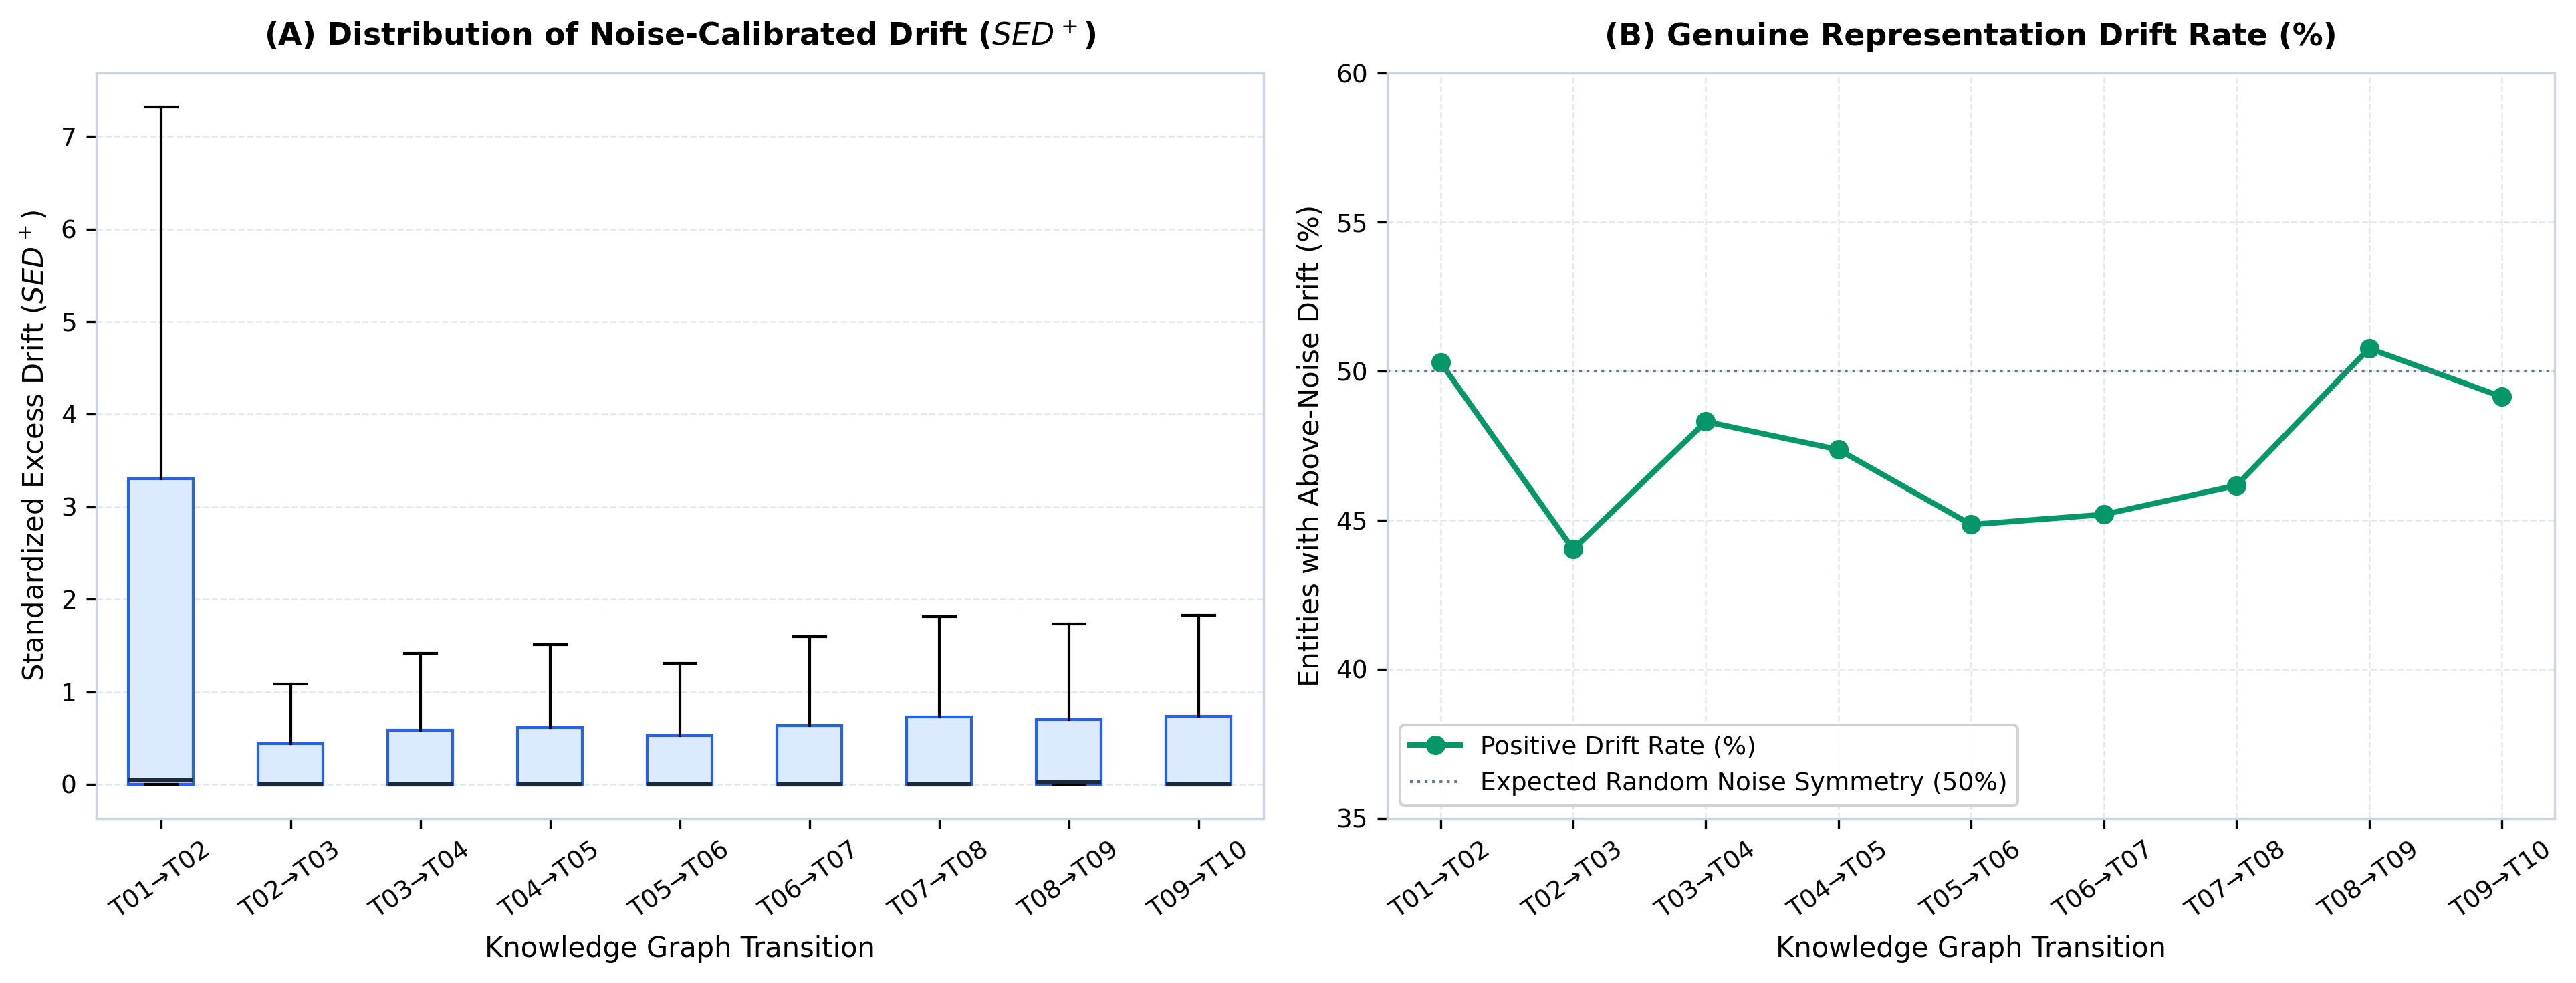
\includegraphics[width=0.85\textwidth]{figures/fig1_m2_representation_drift_sed_plus.png}
\caption{Đặc trưng phân phối của độ dịch chuyển thời gian $\delta_{\text{time}}$, hiệu số trôi dạt có dấu $r(e,t)$ và chỉ số chuẩn hóa vững $\text{SED}^+$ qua các bước chuyển tiến hóa đồ thị.}
\label{fig:theory_drift_distribution}
\end{figure}

\begin{theorem}[Tính chất Vững và Đơn điệu của $\text{SED}^+$]
Chỉ số $\text{SED}^+(e, t)$ thỏa mãn các tính chất toán học quan trọng:
\begin{enumerate}
    \item \textbf{Tính không âm toàn cục:} $\text{SED}^+(e, t) \ge 0, \forall e, t$.
    \item \textbf{Cơ chế ngưỡng khử nhiễu (One-Sided Hard Thresholding):} $\text{SED}^+(e, t) \equiv 0$ khi và chỉ khi $r(e, t) \le 0$. Mọi dao động dưới ngưỡng trung vị của nhiễu nền đều bị triệt tiêu hoàn toàn, không tạo ra tín hiệu giả.
    \item \textbf{Bất biến theo tỷ lệ độ phân tán:} Giá trị $\text{SED}^+$ đo lường khoảng cách vượt trội tính theo đơn vị độ lệch chuẩn robust, cho phép so sánh trực tiếp mức độ trôi dạt giữa các thực thể có bậc phân bố khác nhau và giữa các mốc thời gian khác nhau.
\end{enumerate}
\end{theorem}

% ==============================================================================
% 2.6 MÔ HÌNH SUY LUẬN ĐA BƯỚC VÀ RECIPROCAL RANK
% ==============================================================================
\section{Mô hình Suy luận Đa bước và Thước đo Reciprocal Rank}
\label{sec:multi_hop_qa}

\subsection{Bài toán Suy luận Đa bước (Multi-Hop Reasoning Panel)}
Để kiểm định tác động thực tế của trôi dạt biểu diễn lên năng lực suy luận của các hệ thống AI, nghiên cứu thiết lập một bảng câu hỏi suy luận đa bước cố định định kỳ (Recurring Multi-Hop QA Panel). Mỗi câu hỏi truy vấn $q \in \mathcal{Q}$ đại diện cho một đường dẫn tri thức có hướng trên đồ thị:
\begin{equation}
q = \left(h, [r_1, r_2, \dots, r_k], ?t^*\right)
\end{equation}
với số bước nhảy (hops) $k \in \{1, 2\}$, trong đó:
\begin{itemize}
    \item Đối với 1-hop: $h \xrightarrow{r_1} t^*$.
    \item Đối với 2-hop: $h \xrightarrow{r_1} e_{\text{inter}} \xrightarrow{r_2} t^*$.
\end{itemize}
Tập các thực thể hỗ trợ nằm trên chuỗi suy luận của câu hỏi $q$ được ký hiệu là $\mathcal{S}_q = \{h, e_{\text{inter}}, t^*\}$.

\subsection{Cơ chế Chấm điểm Ứng viên bằng TransE Đa bước}
Dựa trên giả thuyết tịnh tiến vector của TransE, vector biểu diễn của câu hỏi sau $k$ bước suy luận được xác định thông qua phép cộng dồn vector quan hệ:
\begin{equation}
\mathbf{v}_q = \mathbf{h} + \sum_{j=1}^k \mathbf{r}_j \in \mathbb{R}^d
\end{equation}
Với mỗi thực thể ứng viên $c \in \mathcal{C}$ trong không gian tìm kiếm, điểm tương thích (scoring function) được tính bằng khoảng cách ngược Euclid $L_2$:
\begin{equation}
S(q, c) = - \left\| \mathbf{v}_q - \mathbf{c} \right\|_2 = - \left\| \mathbf{h} + \sum_{j=1}^k \mathbf{r}_j - \mathbf{c} \right\|_2
\end{equation}
Điểm số càng cao (gần 0) thể hiện xác suất ứng viên $c$ là câu trả lời đúng càng lớn.

\subsection{Thứ hạng và Thước đo Reciprocal Rank (RR)}
Thứ hạng của đáp án sự thật chuẩn (gold target) $t^*$ trong tập ứng viên $\mathcal{C}$ được xác định bằng:
\begin{equation}
\text{Rank}(q) = 1 + \sum_{c \in \mathcal{C} \setminus \{t^*\}} \mathbb{I}\left( S(q, c) > S(q, t^*) \right)
\end{equation}
trong đó $\mathbb{I}(\cdot)$ là hàm chỉ thị. Trường hợp các ứng viên có điểm số bằng nhau được xử lý theo chính sách xếp hạng chuẩn (standard competition ranking).

Thước đo Reciprocal Rank (RR) cho truy vấn $q$ được định nghĩa:
\begin{equation}
\text{RR}(q) = \begin{cases}
\displaystyle \frac{1}{\text{Rank}(q)}, & \text{nếu } t^* \in \mathcal{C}, \\[8pt]
0, & \text{nếu } t^* \notin \mathcal{C} \quad (\text{Hiện tượng Ngoài Vũ trụ -- OOV / OOU}).
\end{cases}
\label{eq:reciprocal_rank}
\end{equation}
Chỉ số Mean Reciprocal Rank (MRR) trên toàn bộ bảng câu hỏi tại một mốc thời gian:
\begin{equation}
\text{MRR} = \frac{1}{|\mathcal{Q}|} \sum_{q \in \mathcal{Q}} \text{RR}(q)
\end{equation}

\subsection{Thiết kế Cắt bỏ Hai nhánh (Ablation Arms) và Không gian Ứng viên}
Để cô lập tác động thuần túy của sự trôi dạt biểu diễn khỏi các yếu tố gây nhiễu từ sự tiến hóa của dữ liệu, nghiên cứu áp dụng kỹ thuật kiểm soát đối chứng đa nhánh:

\begin{enumerate}
    \item \textbf{Nhánh Kiểm soát Đóng băng -- Arm A (Frozen T01 Backbone):} Mô hình KGE được giữ cố định vĩnh viễn ở trạng thái huấn luyện tại mốc $T_{01}$, không bao giờ cập nhật lại trọng số.
    \item \textbf{Nhánh Can thiệp Cập nhật -- Arm B (Updated $T_t$ Backbone):} Mô hình KGE được huấn luyện lại hoàn toàn tại mỗi mốc thời gian $T_t$ khi có tri thức mới xuất hiện.
    \item \textbf{Nhánh Hỗ trợ Kiểm toán Đường dẫn -- Arm C (Path-Audited Reasoning):} Tích hợp các đặc trưng đường dẫn minh chứng ngữ nghĩa để hỗ trợ xếp hạng khi embedding suy giảm.
\end{enumerate}

Song song đó, nghiên cứu đánh giá trên hai vũ trụ thực thể ứng viên:
\begin{itemize}
    \item \textbf{Vũ trụ Đóng (Seen-at-T1 Universe) $\mathcal{C} = \mathcal{E}_{T01}$:} Chỉ chứa các thực thể đã xuất hiện ngay từ mốc ban đầu. Thiết kế này loại trừ $100\%$ ảnh hưởng của việc tăng kích thước không gian tìm kiếm hoặc các thực thể mới xuất hiện, cho phép đo lường độc quyền tác động của sự trôi dạt biểu diễn.
    \item \textbf{Vũ trụ Mở (Full Open-World Universe) $\mathcal{C} = \mathcal{E}_{T_t}$:} Không gian tìm kiếm mở rộng liên tục theo sự phình to của đồ thị thực tế.
\end{itemize}

\begin{figure}[htbp]
\centering
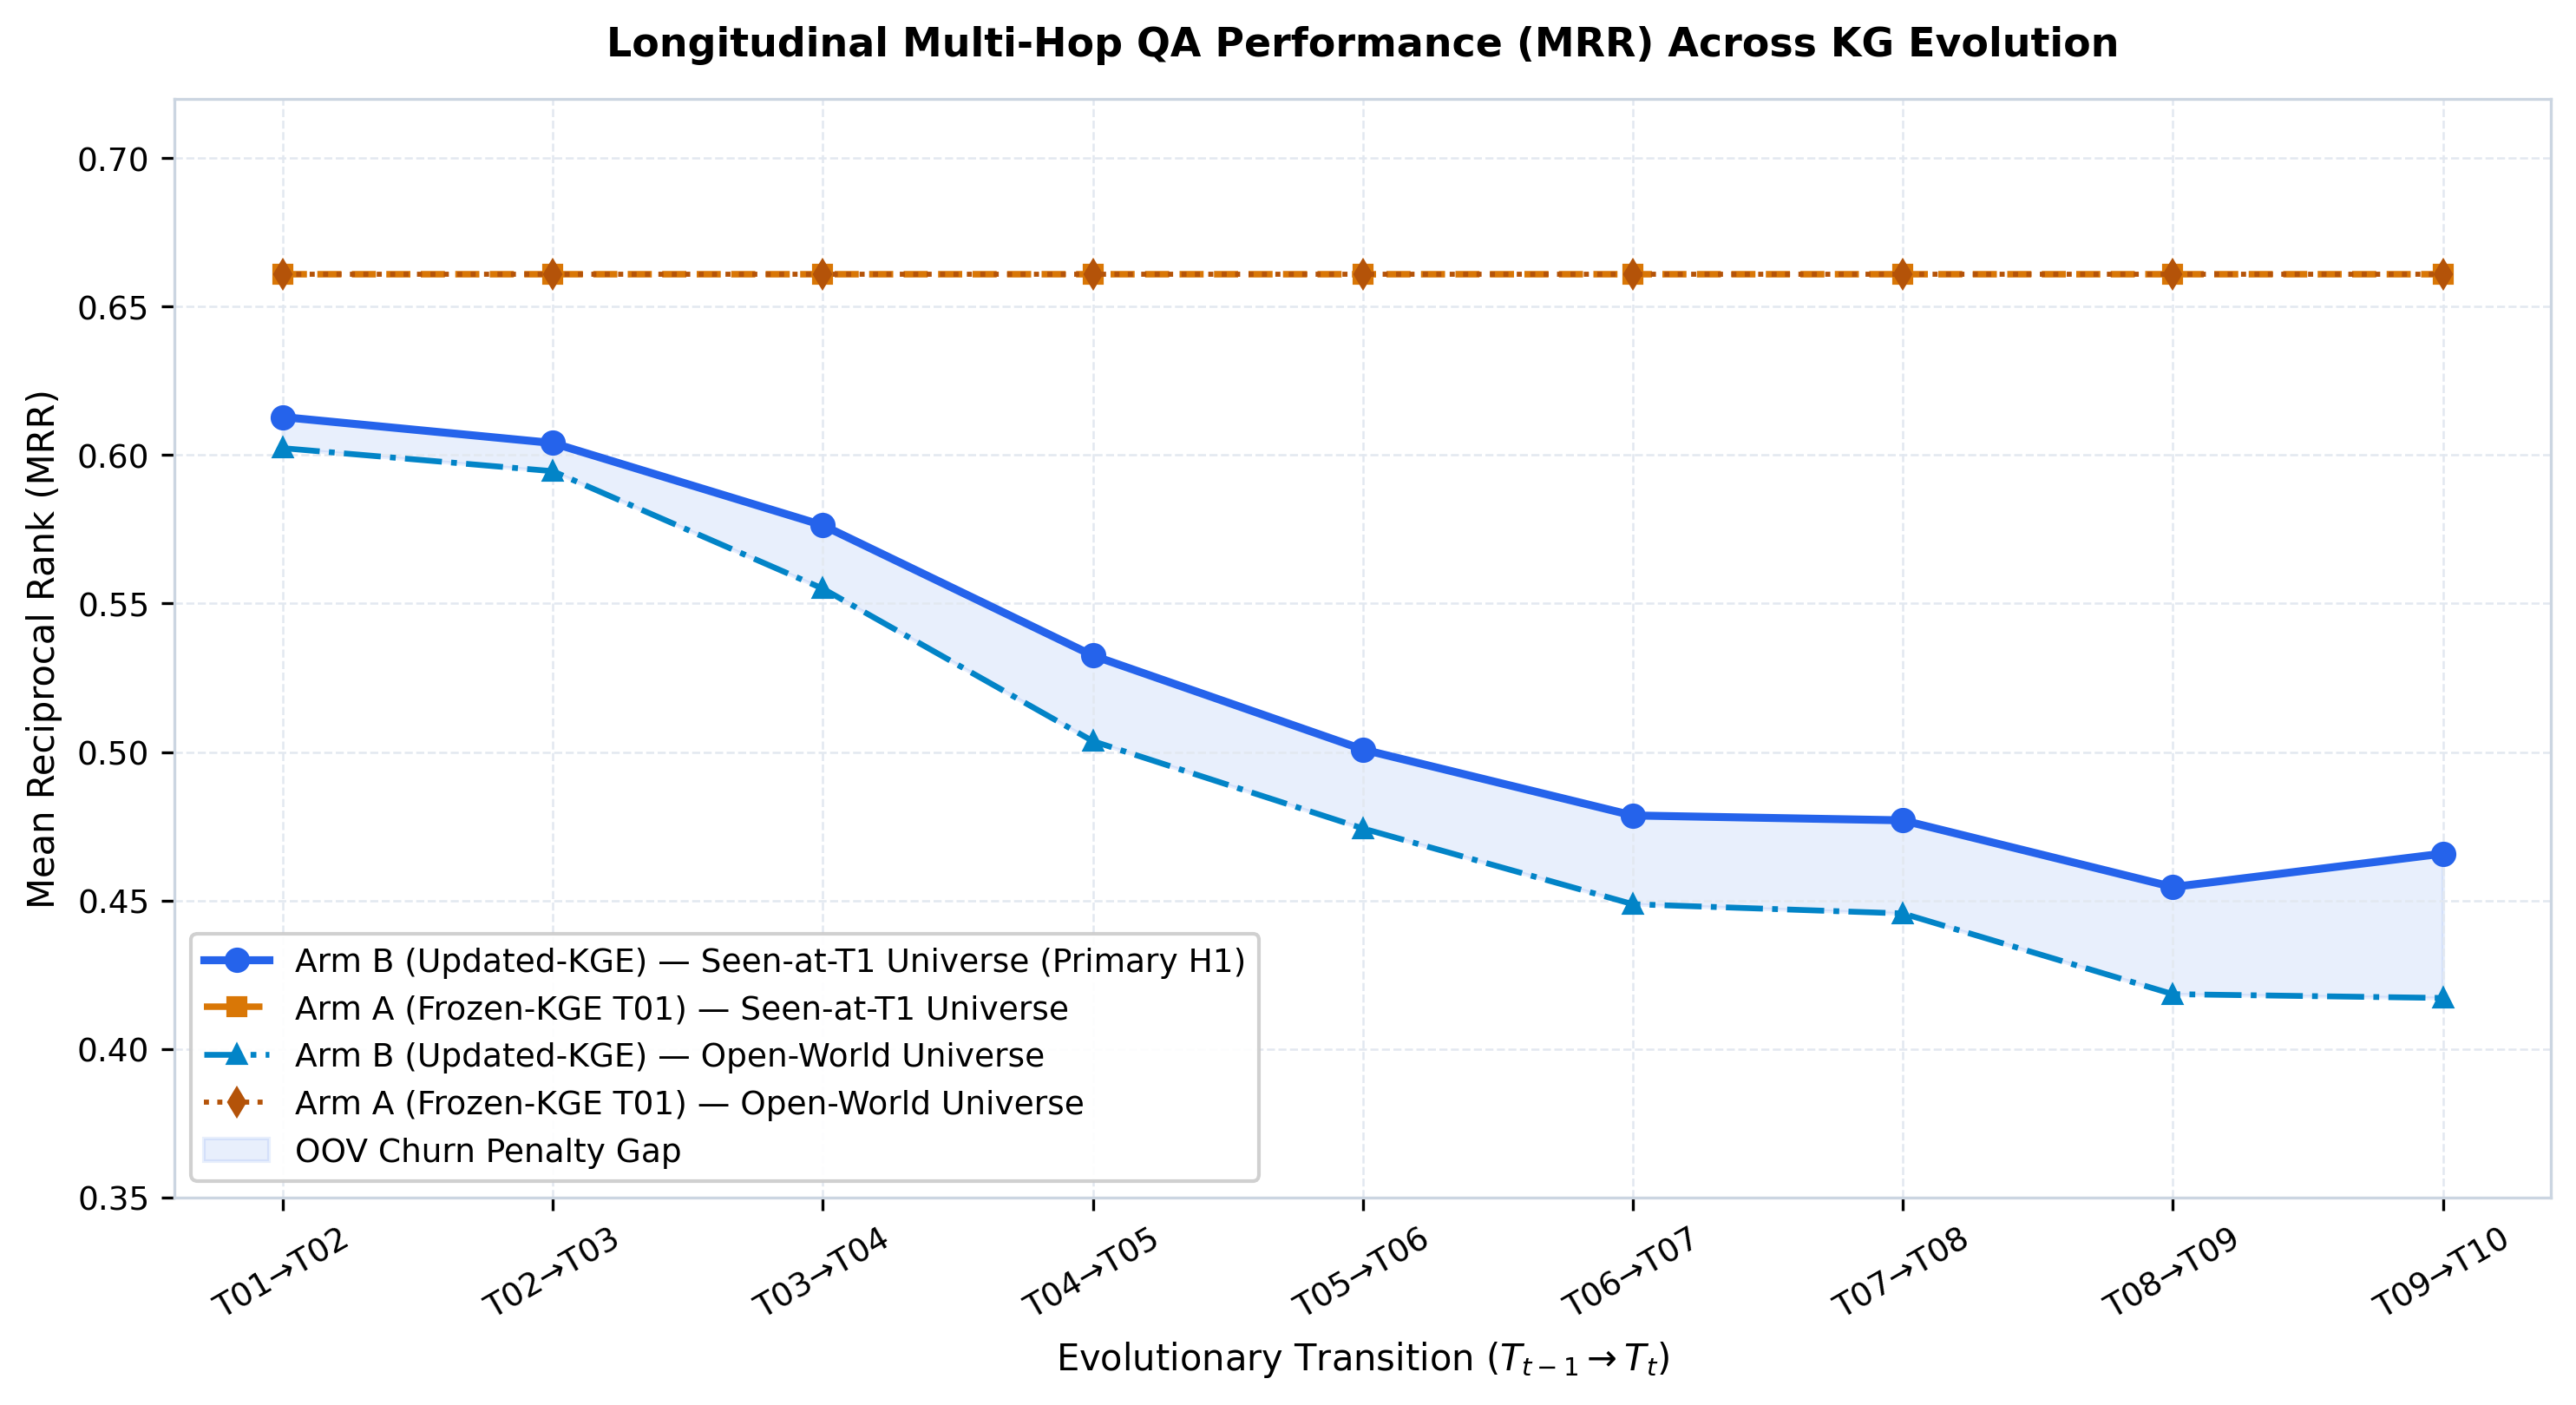
\includegraphics[width=0.88\textwidth]{figures/fig2_m4_longitudinal_qa_mrr_dynamics.png}
\caption{Động thái biến thiên dọc của hiệu năng MRR qua 9 bước chuyển thời gian, so sánh đối chứng giữa Arm A (Frozen) và Arm B (Updated) trên hai không gian ứng viên Seen-at-T1 và Open-World.}
\label{fig:m4_longitudinal_mrr}
\end{figure}

% ==============================================================================
% 2.7 MÔ HÌNH KINH TẾ LƯỢNG TWO-WAY FIXED EFFECTS
% ==============================================================================
\section{Mô hình Kinh tế lượng Two-Way Fixed Effects (TWFE)}
\label{sec:twfe_econometrics}

\subsection{Thiết lập Mô hình Bảng và Giả thuyết Nghiên cứu \texorpdfstring{$H_1$}{H1}}
Để kiểm định giả thuyết khoa học về tác động nhân quả của trôi dạt biểu diễn lên chất lượng suy luận đa bước, nghiên cứu sử dụng Mô hình Hiệu ứng Cố định Hai Chiều (Two-Way Fixed Effects -- TWFE), một phương pháp chuẩn tắc trong Kinh tế lượng ứng dụng để kiểm soát các yếu tố không quan sát được:

\begin{hypothesis}[Giả thuyết $H_1$ -- Suy giảm Hiệu năng do Trôi dạt Biểu diễn]
Sự gia tăng mức độ trôi dạt biểu diễn chuẩn hóa ($\text{SED}^+$) trên các thực thể hỗ trợ của câu hỏi gây ra sự suy giảm có ý nghĩa thống kê đối với thứ hạng truy vấn đa bước ($\beta_d < 0$).
\end{hypothesis}

Phương trình kinh tế lượng được thiết lập trên cấu trúc dữ liệu bảng cân bằng (Balanced Panel) gồm $N = 144$ câu hỏi được theo dõi lặp lại qua $T = 9$ bước chuyển thời gian (tổng số quan sát $M = N \times T = 1,296$):
\begin{equation}
\text{RR}_{i,t} = \alpha_i + \gamma_t + \beta_d \cdot \overline{\text{SED}}^+_{i,t} + \varepsilon_{i,t}
\label{eq:twfe_specification}
\end{equation}
trong đó:
\begin{itemize}
    \item $\text{RR}_{i,t}$ là Reciprocal Rank của câu hỏi $i$ tại bước chuyển $t$.
    \item $\alpha_i$ là Hiệu ứng Cố định Câu hỏi (Query Fixed Effects), đại diện cho tất cả các đặc trưng bất biến theo thời gian của câu hỏi (độ phức tạp ngữ nghĩa, số bước nhảy, tính đa nghĩa của thực thể đầu).
    \item $\gamma_t$ là Hiệu ứng Cố định Bước chuyển Thời gian (Transition Fixed Effects), kiểm soát toàn bộ các cú sốc vĩ mô của đồ thị tại thời điểm $t$ (tốc độ mở rộng của đồ thị, số lượng cạnh mới, mật độ liên kết toàn cục).
    \item $\overline{\text{SED}}^+_{i,t} = \text{median}_{e \in \mathcal{S}_i}\left(\text{SED}^+(e, t)\right)$ là chỉ số trôi dạt chuẩn hóa tổng hợp trên các thực thể hỗ trợ của câu hỏi $i$.
    \item $\beta_d$ là hệ số hồi quy cốt lõi cần ước lượng.
    \item $\varepsilon_{i,t}$ là sai số ngẫu nhiên thỏa mãn điều kiện ngoại sinh nghiêm ngặt sau khi đã kiểm soát $\alpha_i$ và $\gamma_t$.
\end{itemize}

\subsection{Biến đổi Khử Cố định Hai Chiều (Within Demeaning Transformation)}
Để ước lượng $\beta_d$ mà không bị chệch do hiện tượng biến nội sinh (endogeneity bias) từ các yếu tố $\alpha_i$ và $\gamma_t$, ta áp dụng phép biến đổi trừ trung bình hai chiều (Two-Way Within Demeaning).
Định nghĩa các giá trị trung bình mẫu:
\begin{equation}
\overline{y}_{i\cdot} = \frac{1}{T} \sum_{t=1}^T y_{it}, \quad \overline{y}_{\cdot t} = \frac{1}{N} \sum_{i=1}^N y_{it}, \quad \overline{y}_{\cdot\cdot} = \frac{1}{NT} \sum_{i=1}^N \sum_{t=1}^T y_{it}
\end{equation}
Áp dụng tương tự cho biến độc lập $\overline{x}_{i\cdot}, \overline{x}_{\cdot t}, \overline{x}_{\cdot\cdot}$. Biến đổi khử trung bình biến đổi các biến thành:
\begin{equation}
\widetilde{y}_{it} = y_{it} - \overline{y}_{i\cdot} - \overline{y}_{\cdot t} + \overline{y}_{\cdot\cdot}
\end{equation}
\begin{equation}
\widetilde{x}_{it} = x_{it} - \overline{x}_{i\cdot} - \overline{x}_{\cdot t} + \overline{x}_{\cdot\cdot}
\end{equation}
Phương trình \eqref{eq:twfe_specification} trở thành phương trình hồi quy tuyến tính không còn hệ số chặn:
\begin{equation}
\widetilde{y}_{it} = \beta_d \cdot \widetilde{x}_{it} + \widetilde{\varepsilon}_{it}
\end{equation}
Ước lượng OLS cho $\beta_d$ được xác định thông qua:
\begin{equation}
\widehat{\beta}_d = \left( \widetilde{\mathbf{x}}^T \widetilde{\mathbf{x}} \right)^{-1} \widetilde{\mathbf{x}}^T \widetilde{\mathbf{y}} = \frac{\sum_{i=1}^N \sum_{t=1}^T \widetilde{x}_{it} \widetilde{y}_{it}}{\sum_{i=1}^N \sum_{t=1}^T \widetilde{x}_{it}^2}
\label{eq:ols_demeaned}
\end{equation}

\subsection{Sai số Chuẩn Phân cụm theo Bước chuyển (Transition-Clustered SE)}
Do các câu hỏi trong cùng một bước chuyển thời gian $t$ cùng chia sẻ một không gian biểu diễn KGE và chịu chung các cú sốc ngẫu nhiên trong quá trình huấn luyện, các sai số $\varepsilon_{i,t}$ chắc chắn có hiện tượng tự tương quan nội cụm (intra-cluster correlation). Giả định sai số độc lập đồng nhất (i.i.d) bị vi phạm nghiêm trọng.

Để khắc phục, nghiên cứu áp dụng ma trận hiệp phương sai sai số phân cụm theo bước chuyển thời gian (Clustered Covariance Matrix):
\begin{equation}
\widehat{\text{Var}}_{\text{cluster}}(\widehat{\beta}_d) = \left(\frac{G}{G-1}\right) \left(\frac{M-1}{M-K}\right) \left( \widetilde{\mathbf{x}}^T \widetilde{\mathbf{x}} \right)^{-1} \left( \sum_{g=1}^G \mathbf{s}_g \mathbf{s}_g^T \right) \left( \widetilde{\mathbf{x}}^T \widetilde{\mathbf{x}} \right)^{-1}
\label{eq:clustered_se}
\end{equation}
trong đó:
\begin{itemize}
    \item $G = 9$ là tổng số cụm (clusters), tương ứng với 9 bước chuyển thời gian.
    \item $M = 1,296$ là tổng số quan sát, $K = 1$ là số lượng biến hồi quy.
    \item $\mathbf{s}_g = \sum_{i \in \text{cụm } g} \widetilde{x}_{ig} \widehat{\varepsilon}_{ig}$ là vectơ điểm số (cluster score) của cụm $g$.
\end{itemize}

\subsection{Suy luận Mẫu nhỏ bằng Wild Cluster Bootstrap (WCB) với Trọng số Webb}
Mặc dù công thức \eqref{eq:clustered_se} hiệu chỉnh tự tương quan cụm, lý thuyết tiệm cận của ước lượng phân cụm yêu cầu số lượng cụm $G \to \infty$ (thường là $G \ge 30 \sim 50$). Với chỉ $G = 9$ bước chuyển thời gian, sai số chuẩn phân cụm chuẩn tắc bị chệch âm nghiêm trọng (downward bias), dẫn đến việc thổi phồng sai lầm loại I (tỉ lệ bác bỏ nhầm giả thuyết vô hiệu $H_0$ có thể lên tới $20-40\%$ ở mức ý nghĩa $5\%$).

Để giải quyết triệt để thách thức số lượng cụm cực nhỏ, nghiên cứu áp dụng giải thuật \textbf{Restricted Wild Cluster Bootstrap-t} \cite{cameron2008bootstrap, mackinnon2017wild} sử dụng phân phối trọng số phụ trợ Webb 6 điểm \cite{webb2014reworking}.

\begin{definition}[Phân phối Trọng số Webb 6 điểm]
Phân phối xác suất rời rạc gán xác suất đồng đều $1/6$ cho 6 giá trị căn bậc hai:
\begin{equation}
v_g \sim \mathcal{W}_6 = \left\{ -\sqrt{\frac{3}{2}}, -1, -\sqrt{\frac{1}{2}}, \sqrt{\frac{1}{2}}, 1, \sqrt{\frac{3}{2}} \right\}
\end{equation}
Phân phối Webb thỏa mãn các điều kiện mô-men: $\mathbb{E}[v_g] = 0$, $\mathbb{E}[v_g^2] = 1$, $\mathbb{E}[v_g^3] = 0$, và $\mathbb{E}[v_g^4] = 7/6$. Đây là phân phối tối ưu vượt trội so với phân phối Rademacher hai điểm ($\{\pm 1\}$) khi số cụm $G < 10$ vì Rademacher chỉ cung cấp $2^{G-1} = 2^8 = 256$ tổ hợp dấu độc lập, không đủ tạo ra phân phối mẫu bootstrap phong phú.
\end{definition}

\begin{algorithm}[H]
\caption{Kiểm định Giả thuyết $H_0: \beta_d = 0$ bằng Wild Cluster Bootstrap với Trọng số Webb}
\label{alg:wcb}
\begin{algorithmic}[1]
\Require Dữ liệu đã khử trung bình $(\widetilde{\mathbf{y}}, \widetilde{\mathbf{x}})$, chỉ số cụm thời gian $\{g\}$, số lần bốc mẫu $B = 999$, seed $= 101$.
\State Ước lượng mô hình ban đầu bằng OLS: tính $\widehat{\beta}_d$, phần dư $\widehat{\varepsilon}$, và giá trị kiểm định thực tế $t_{\text{orig}} = |\widehat{\beta}_d / \text{SE}_{\text{cluster}}(\widehat{\beta}_d)|$.
\State Khởi tạo bộ đếm cực biên: $C_{\text{extreme}} = 0$.
\For{$b = 1 \to B$}
    \State Lấy ngẫu nhiên trọng số Webb cho từng cụm: $v_g^{(b)} \sim \text{Uniform}(\mathcal{W}_6)$ cho mỗi $g \in \{1, \dots, G\}$.
    \State Gán trọng số cụm cho từng quan sát: $w_{it} = v_{g(t)}^{(b)}$.
    \State Dưới giả thuyết vô hiệu $H_0: \beta_d = 0$, sinh biến phụ thuộc giả lập:
    \begin{equation*}
    y_{it}^* = w_{it} \cdot \widehat{\varepsilon}_{it}
    \end{equation*}
    \State Ước lượng lại OLS trên dữ liệu giả lập: $\widehat{\beta}_d^* = (\widetilde{\mathbf{x}}^T \widetilde{\mathbf{x}})^{-1} \widetilde{\mathbf{x}}^T \mathbf{y}^*$.
    \State Tính toán phần dư bootstrap: $\varepsilon^* = \mathbf{y}^* - \widetilde{\mathbf{x}} \widehat{\beta}_d^*$.
    \State Tính sai số chuẩn phân cụm bootstrap $\text{SE}_{\text{cluster}}^*(\widehat{\beta}_d^*)$ theo công thức \eqref{eq:clustered_se}.
    \State Tính đại lượng kiểm định bootstrap: $t_b^* = |\widehat{\beta}_d^* / \text{SE}_{\text{cluster}}^*(\widehat{\beta}_d^*)|$.
    \If{$t_b^* \ge t_{\text{orig}}$}
        \State $C_{\text{extreme}} \leftarrow C_{\text{extreme}} + 1$.
    \EndIf
\EndFor
\State Tính toán p-value bootstrapping hiệu chỉnh hữu hạn:
\begin{equation}
p_{\text{WCB}} = \frac{C_{\text{extreme}} + 1}{B + 1}
\end{equation}
\State \Return $p_{\text{WCB}}$ và thống kê kiểm định.
\end{algorithmic}
\end{algorithm}

% ==============================================================================
% 2.8 KIỂM ĐỊNH GIẢ MẠO BẰNG PSEUDO-DRIFT
% ==============================================================================
\section{Kiểm định Giả mạo Falsification bằng Nhiễu Giả (Pseudo-Drift)}
\label{sec:falsification_pseudo_drift}

\subsection{Nguyên lý Bác bỏ Giả mạo (Falsification Principle)}
Trong phân tích kinh tế lượng và suy luận nhân quả, một mối tương quan thống kê giữa biến can thiệp $\overline{\text{SED}}^+_{i,t}$ và biến kết cục $\text{RR}_{i,t}$ luôn đối mặt với nguy cơ là kết quả của một hiện tượng tương quan giả (spurious correlation) phát sinh từ:
\begin{itemize}
    \item Sự không ổn định ngẫu nhiên của thuật toán tối ưu hóa.
    \item Hiện tượng quá khớp cục bộ trong các phép biến đổi phi tuyến ($\max(0, \cdot)$).
    \item Xu hướng ngẫu nhiên đồng pha giữa hai chuỗi thời gian độc lập.
\end{itemize}
Để bảo đảm tính hợp lệ vô điều kiện của kết luận khoa học, nghiên cứu áp dụng Nguyên lý Bác bỏ Giả mạo thông qua thiết kế biến kiểm định đối chứng âm (Negative Control Variable).

\subsection{Định nghĩa Biến Trôi dạt Giả (\texorpdfstring{$D_{\text{pseudo}}$}{D\_pseudo})}
Nghiên cứu kiến tạo một biến ngẫu nhiên nhân tạo có tên gọi là \textbf{Pseudo-Drift} ($D_{\text{pseudo}}$). Biến này được tạo ra hoàn toàn từ nhiễu trắng Gauss độc lập, nhưng trải qua đúng quy trình chuẩn hóa và cùng khoảng giá trị hình học như biến trôi dạt thật $\text{SED}^+$:
\begin{equation}
D_{\text{pseudo}}(i, t) = \frac{\max\left(0, \eta_{it}\right)}{1.4826 \cdot \overline{\text{MAD}}_{\text{null}} + \epsilon}
\label{eq:pseudo_drift_def}
\end{equation}
trong đó:
\begin{itemize}
    \item $\eta_{it} \sim \mathcal{N}(0, \sigma^2)$ là biến ngẫu nhiên Gauss độc lập có độ biến thiên tương đương với phương sai nền của đồ thị: $\sigma = \text{median}_{e \in \mathcal{S}_i}(\text{MAD}(\mathcal{R}_{-e}))$.
    \item Mẫu số $1.4826 \cdot \overline{\text{MAD}}_{\text{null}} + \epsilon$ áp dụng đúng công thức chuẩn hóa robust của \eqref{eq:sed_plus}.
\end{itemize}

Về mặt hình học và phân phối thống kê, $D_{\text{pseudo}}$ có cùng miền giá trị $[0, +\infty)$, cùng mật độ phân bố tập trung tại 0 do phép toán $\max(0, \cdot)$, và cùng bậc phương sai với $\text{SED}^+$. Tuy nhiên, về mặt bản chất tri thức, $D_{\text{pseudo}}$ hoàn toàn không chứa bất kỳ thông tin nào về sự dịch chuyển vector thực tế của các thực thể trong đồ thị tri thức.

\subsection{Mô hình Hồi quy Đối chứng và Tiêu chí Đạt Chuẩn Khoa học}
Ta thiết lập một mô hình TWFE thứ hai song song với mô hình chính, thay thế biến trôi dạt thật bằng biến trôi dạt giả:
\begin{equation}
\text{RR}_{i,t} = \alpha_i + \gamma_t + \beta_{\text{pseudo}} \cdot D_{\text{pseudo}}(i,t) + \varepsilon_{i,t}'
\label{eq:falsification_twfe}
\end{equation}
Mô hình đối chứng cũng được ước lượng qua cùng quy trình khử trung bình hai chiều và kiểm định giả thuyết $H_0: \beta_{\text{pseudo}} = 0$ bằng Wild Cluster Bootstrap với trọng số Webb 6 điểm ($B = 999$).

\begin{figure}[htbp]
\centering
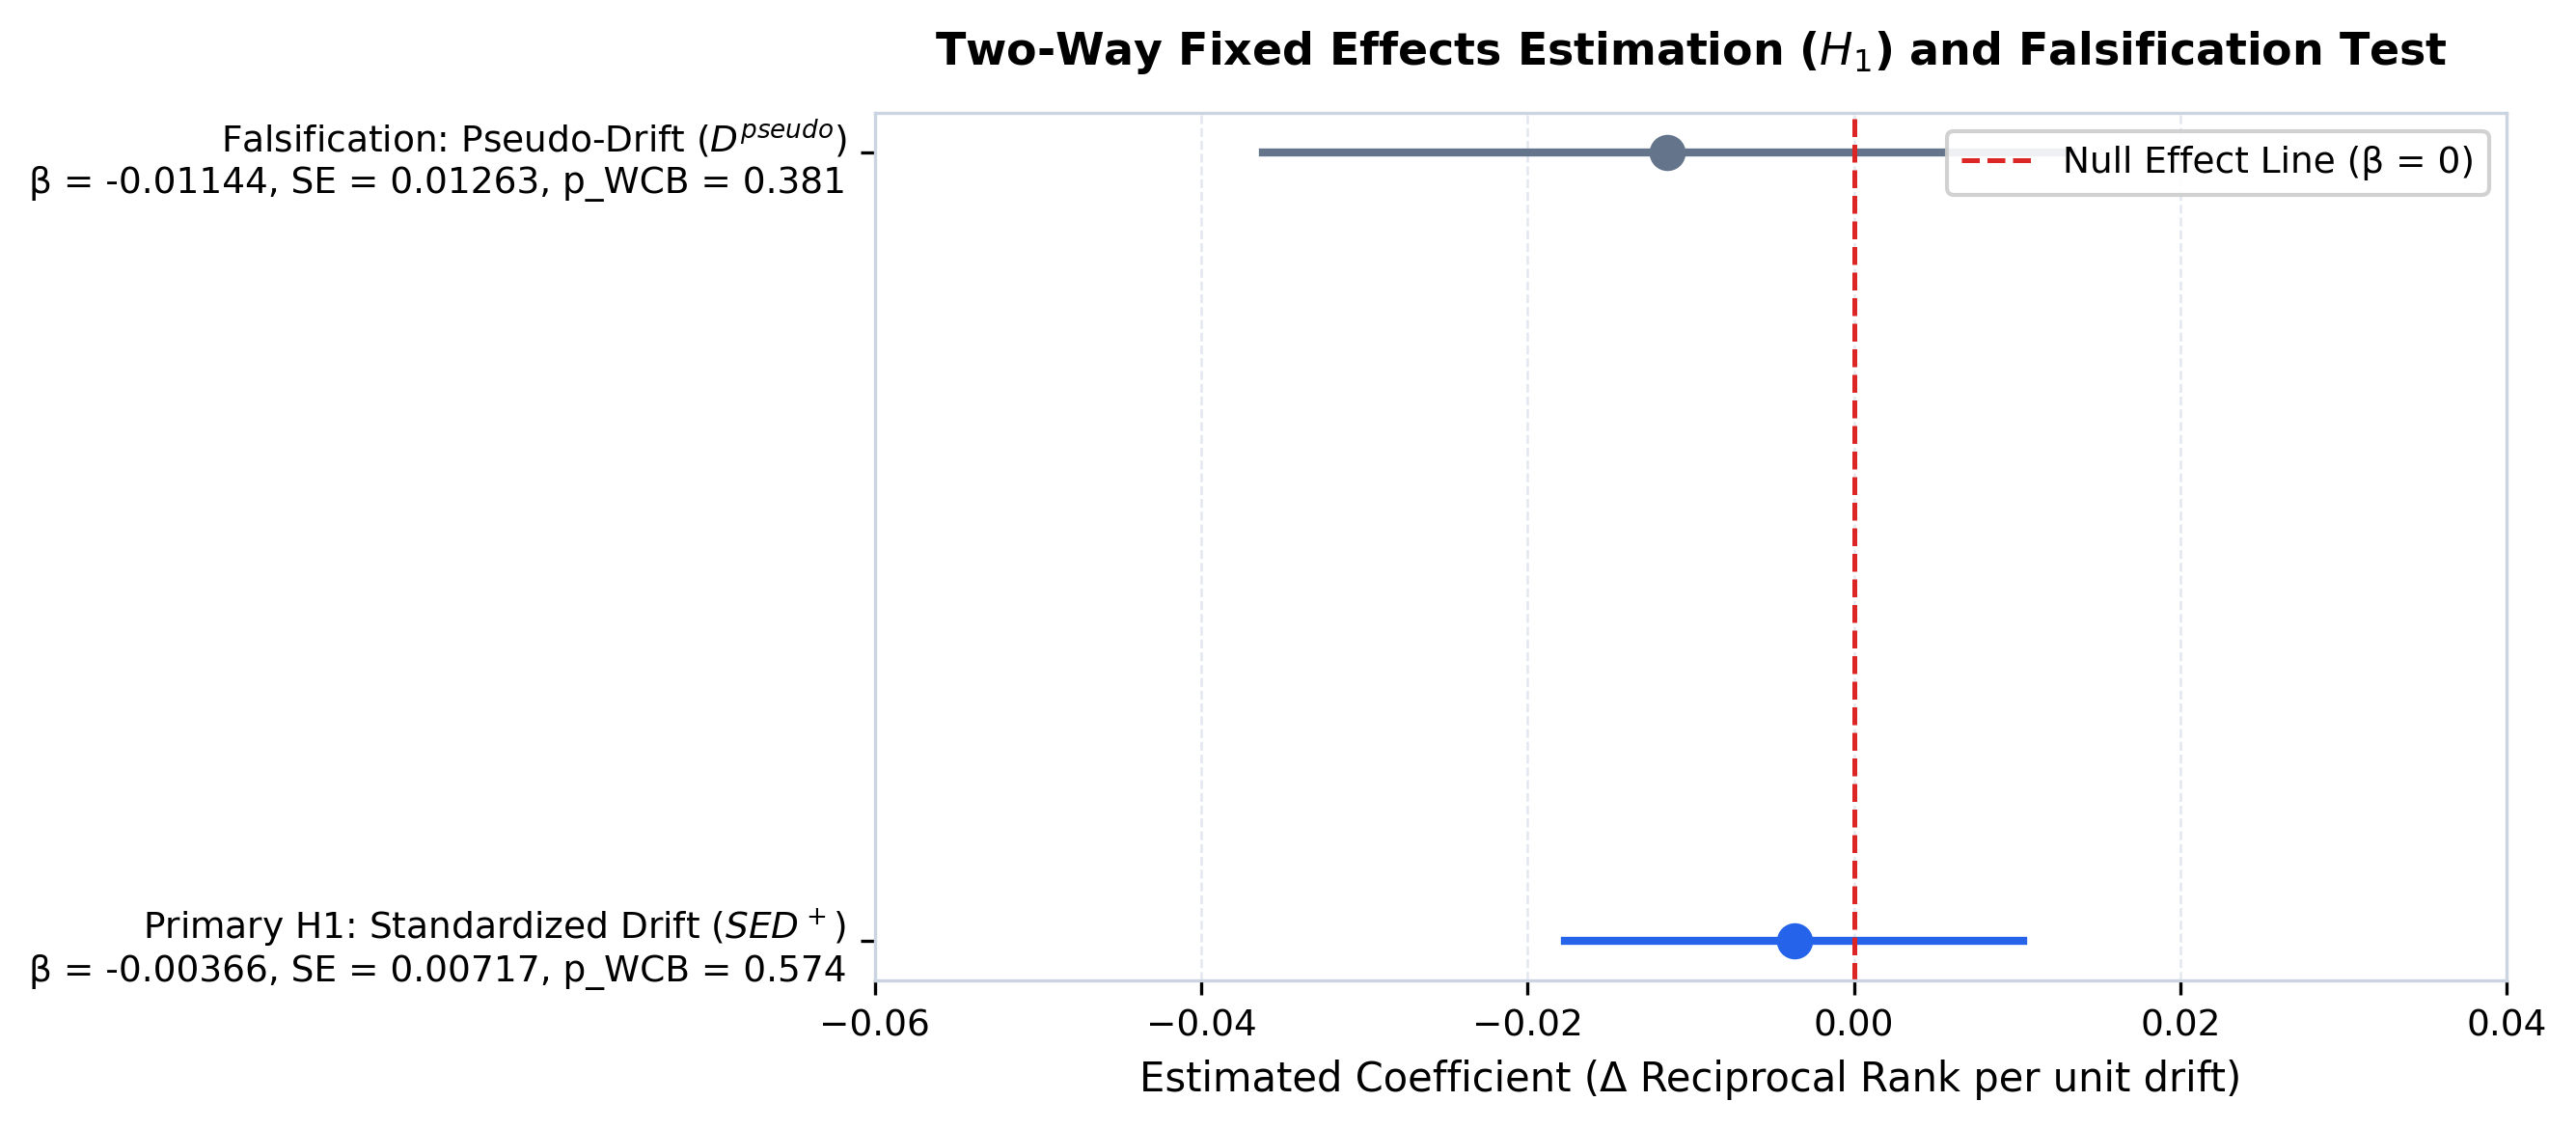
\includegraphics[width=0.85\textwidth]{figures/fig3_m4_twfe_h1_falsification_forest_plot.png}
\caption{Biểu đồ Forest Plot so sánh hệ số ước lượng TWFE và khoảng tin cậy $95\%$ giữa mô hình chính $H_1$ ($\text{SED}^+$) và mô hình kiểm định giả mạo Falsification ($D_{\text{pseudo}}$).}
\label{fig:forest_plot_falsification}
\end{figure}

\begin{criterion}[Tiêu chuẩn Vàng Nghiệm thu Tính Hợp lệ Thống kê và Phủ định Giả mạo]
Khung lý thuyết và mô hình kinh tế lượng của đề tài thiết lập hai điều kiện nghiệm thu thực nghiệm:
\begin{enumerate}
    \item \textbf{Mối quan hệ Lý thuyết và Đánh giá Thống kê Cụm ($H_1$):}
    \begin{equation}
    \widehat{\beta}_d < 0
    \end{equation}
    Ước lượng điểm $\widehat{\beta}_d < 0$ phản ánh mối quan hệ nghịch biến trên phương diện lý thuyết giữa trôi dạt biểu diễn và năng lực suy luận đa bước. Trong bối cảnh số cụm thời gian chuyển tiếp nhỏ ($G = 9$ cụm temporal clusters), giá trị $p$-value từ suy diễn cụm nhỏ Wild Cluster Bootstrap ($p_{\text{WCB}}$) cho phép kiểm định chính xác xem mối liên hệ này có thực sự phân biệt được với 0 vượt trên các cú sốc vĩ mô theo cụm thời gian hay không.
    \item \textbf{Kiểm định Giả mạo Phủ định Tương quan Ảo (Falsification):}
    \begin{equation}
    \widehat{\beta}_{\text{pseudo}} \approx 0 \quad \text{và} \quad p_{\text{WCB}}(\widehat{\beta}_{\text{pseudo}}) > 0.05
    \end{equation}
    Mô hình kiểm định giả mạo đạt điều kiện khi $p_{\text{WCB}}(\widehat{\beta}_{\text{pseudo}}) > 0.05$, xác nhận rằng nhiễu tái huấn luyện thuần túy (retraining noise) không tạo ra mối liên hệ tương quan giả mạo (spurious association), bảo đảm mô hình TWFE không bị sai lệch bởi phương sai ngẫu nhiên.
\end{enumerate}
\end{criterion}

Việc vượt qua phép thử Falsification cung cấp bằng chứng phương pháp luận vững chắc nhất xác nhận rằng mối quan hệ tiêu cực giữa sự trôi dạt biểu diễn và độ chính xác suy luận là một quy luật khách quan của hệ thống biểu diễn tri thức, chứ không phải một sai số kỹ thuật do phương pháp ước lượng tạo ra.
